\documentclass[a4paper]{article}
\renewcommand{\familydefault}{\sfdefault}
%Seitenränder definieren
\usepackage[right=4.0cm,left=3.3cm, bottom=3.9cm, top=4.1cm, footskip=2.1cm, headsep=2.0cm]{geometry}
\usepackage[utf8x]{inputenc}
\usepackage[T1]{fontenc}
\usepackage{palatino}
\linespread{1.25}
\usepackage{microtype}
\usepackage[english]{babel}
%More citations
\usepackage{natbib}
%better urls mit \url{}
\usepackage{url}
\usepackage{lastpage}
%code
\usepackage{listings}

%more colors
\usepackage{soul}

%Force figure to be placed “HERE”
\usepackage{float} 

%folgende Zeilen sind für Kapitelüberschriften
\usepackage[rigidchapters]{titlesec}
\usepackage{blindtext}
\titleformat{\chapter}
{\normalfont\LARGE}
{\makebox[3pc][l]{\LARGE\thechapter\hfil\rule[-6pt]{0.5pt}{2pc}}}
{0pt}
{\LARGE}
\titlespacing*{\chapter}{0pt}{0pt}{82pt}

%Csv -> Latex
\usepackage{csvsimple}

%Für Graphiken 
\usepackage{tikz}
\usetikzlibrary{plotmarks}
\usetikzlibrary{positioning,shapes,shadows,arrows}
\usepackage{graphicx}

%Paket gibt einige Optionen mehr bei Tabellen (wird eher nicht verwendet)
\usepackage{array}

%\usepackage{stdpage}
%test wegen anzahl zeilen pro seite
%Paket für Zeilenabstände
\usepackage{setspace}
%\onehalfspacing
\usepackage{multirow}
%Paket gibt mehr Kontrolle über die Captions (Bildunterschriften) bei Abbildungen
\usepackage[labelfont=bf,format=hang,font=footnotesize,justification=raggedright,singlelinecheck=false]{caption}

%Helvetia (Arial) Verwenden WICHTIG: Beide folgenden Zeilen kopieren!
%\usepackage[scaled]{helvet} %
%\renewcommand*\familydefault{\sfdefault} %%

% Abschalten des Einrückens bei neuen Absätzen (manuell, nach Tabellen, Abbildungen, etc.)
\setlength{\parindent}{0pt}
\hyphenation{}

% New Page before section
\newcommand{\sectionbreak}{\clearpage}

\usepackage{color}
\usepackage{lstautogobble}  % Fix relative indenting
\usepackage{zi4}  

\definecolor{color0}{rgb}{0,0,0}% black
\definecolor{color1}{rgb}{0.22,0.45,0.70}% light blue
\definecolor{color2}{rgb}{0.45,0.45,0.45}% dark grey
\definecolor{mygreen}{rgb}{0,0.6,0}
\definecolor{mygray}{rgb}{0.5,0.5,0.5}
\definecolor{myblue}{RGB}{40,58,93}
\definecolor{codebackground}{RGB}{221, 222, 223}
\definecolor{codechanged}{rgb}{0.8, 0.0, 0.0}


\definecolor{bluekeywords}{rgb}{0.13, 0.13, 1}
\definecolor{greencomments}{rgb}{0, 0.5, 0}
\definecolor{redstrings}{rgb}{0.9, 0, 0}
\definecolor{graynumbers}{rgb}{0.5, 0.5, 0.5}

\lstset{
    autogobble,
    columns=fullflexible,
    showspaces=false,
    showtabs=false,
    breaklines=true,
    showstringspaces=false,
    breakatwhitespace=true,
    commentstyle=\color{greencomments},
    keywordstyle=\color{bluekeywords},
    stringstyle=\color{redstrings},
    numberstyle=\color{graynumbers},
    basicstyle=\ttfamily\footnotesize,
    frame=l,
    framesep=12pt,
    xleftmargin=12pt,
    tabsize=4,
    captionpos=b
}


% \lstset{ %
%   backgroundcolor=\color{codebackground},   % choose the background color; you must add \usepackage{color} or \usepackage{xcolor}
%   breakatwhitespace=false,         % sets if automatic breaks should only happen at whitespace
%   breaklines=true,                 % sets automatic line breaking
%   captionpos=b,                    % sets the caption-position to bottom
%   commentstyle=\color{mygreen},    % comment style
%   deletekeywords={...},            % if you want to delete keywords from the given language
%   escapeinside={\%*}{*)},          % if you want to add LaTeX within your code
%   extendedchars=true,              % lets you use non-ASCII characters; for 8-bits encodings only, does not work with UTF-8
%   frame=single,	                   % adds a frame around the code
%   keepspaces=true,                 % keeps spaces in text, useful for keeping indentation of code (possibly needs columns=flexible)
%   keywordstyle=\color{blue},       % keyword style
%   showspaces=false,                % show spaces everywhere adding particular underscores; it overrides 'showstringspaces'
%   showstringspaces=false,          % underline spaces within strings only
%   showtabs=false,                  % show tabs within strings adding particular underscores
%   stepnumber=2,                    % the step between two line-numbers. If it's 1, each line will be numbered
%   stringstyle=\color{mymauve},     % string literal style
%   tabsize=2,	                   % sets default tabsize to 2 spaces
%   title=\lstname,                   % show the filename of files included with \lstinputlisting; also try caption instead of title
%   moredelim=**[is][\color{codechanged}]{**@}{@**}, %Rot für Änderungen
%   moredelim=**[is][\color{myblue}]{***@}{@***}, %einfaches blau
%   moredelim=**[is][\color{mygreen}]{*@}{@*},%einfaches Grün
% }

%Aktives Inhaltsverzeichnis und links
\usepackage{hyperref}
\hypersetup{
    colorlinks,
    citecolor=black,
    filecolor=black,
    linkcolor=black,
    urlcolor=black
}

\usepackage{fancyhdr}
\pagestyle{fancy}
\fancypagestyle{plain}{}
\fancyhf{}
\fancyfoot{} % clear all footer fields


\renewcommand{\sectionmark}[1]{\markboth{#1}{}}

\renewcommand{\footrulewidth}{0.1pt} % Create a rule above the page number
\fancyfoot[R]{\textcolor{color1}\thepage  \textcolor{color2}{/\pageref{LastPage}}}
\fancyhead[L]{}
\fancyhead[R]{}
\fancyhead[C]{
\includegraphics[width=15cm]{header.png}}

\pagestyle{fancy}

\begin{document}

\begin{titlepage}
  \begin{center}
      \vspace*{1cm}
          
      
      {\fontsize{48}{48}\selectfont \textcolor{myblue}{Offensive Security}}
          
      \vspace{0.5cm}
      {\fontsize{28}{28}\selectfont \textcolor{myblue}{OSWE Exam Documentation}}
          
      \vspace{1.5cm}
          
      v.1.0

      \vspace{1cm}

      {\fontsize{16}{16}\selectfont bing.ecnu@gmai.com}

      \vspace{1cm}

      {\fontsize{20}{20}\selectfont OSID: XXXXX}

      \vfill
          
      
\includegraphics[width=9cm]{offsec.png}

      \vfill
      
      \copyright
          
      All rights reserved to Offensive Security, 2020.\\
      No part of this publication, in whole or in part, may be reproduced, copied, transferred or any other right reserved to its copyright owner, 
      including photocopying and all other copying, any transfer or transmission using any network or other means of communication, any broadcast
       for distant learning, in any form or by any means such as any information storage, transmission or retrieval system, without prior written
        permission from Offensive-Security.
      
          
      \vspace{0.8cm}
  
  \end{center}
  \thispagestyle{fancy}
\end{titlepage}


\tableofcontents


\section{Offensive-Security OSWE Exam Documentation}

https://github.com/madneal/oswe-report-teplate
\\

The Offensive Security OSWE exam documentation contains all efforts that were conducted in order to pass the Offensive Security Web Expert exam. This report will be graded from a standpoint of correctness and fullness to all aspects of the exam. The purpose of this report is to ensure that the student has the technical knowledge required to pass the qualifications for the Offensive Security Web Expert certification.
\\
The student will be required to fill out this exam documentation fully and to include the following sections:

\begin{itemize}
  \item Methodology walkthrough and detailed outline of steps taken
  \item Each finding with included screenshots, walkthrough, sample code, and proof.txt if applicable.
  \item Any additional items that were not included
\end{itemize}

\section{192.168.XX.XX}

\subsection{Local.txt / Proof.txt }
Provide the contents of local.txt and proof.txt

\subsection{Vulnerability 1}
Provide the method and code used to find the vulnerability 1.

\subsection{Vulnerability 2}
Provide the method and code used to find the vulnerability 2.

\subsection{Vulnerability X}
Provide the method and code used to find the vulnerability X

\subsection{PoC Code}
Provide the final proof of concept code used to gain access to the server.

\begin{lstlisting}[language=Python]
  import numpy as np
      
  def incmatrix(genl1,genl2):
      m = len(genl1)
      n = len(genl2)
      M = None #to become the incidence matrix
      VT = np.zeros((n*m,1), int)  #dummy variable
      
      #compute the bitwise xor matrix
      M1 = bitxormatrix(genl1)
      M2 = np.triu(bitxormatrix(genl2),1) 
  
      for i in range(m-1):
          for j in range(i+1, m):
              [r,c] = np.where(M2 == M1[i,j])
              for k in range(len(r)):
                  VT[(i)*n + r[k]] = 1;
                  VT[(i)*n + c[k]] = 1;
                  VT[(j)*n + r[k]] = 1;
                  VT[(j)*n + c[k]] = 1;
                  
                  if M is None:
                      M = np.copy(VT)
                  else:
                      M = np.concatenate((M, VT), 1)
                  
                  VT = np.zeros((n*m,1), int)
      
      return M
  \end{lstlisting}

\begin{lstlisting}[language=Java][example.java]

import java.util.Scanner;

public class HelloWorld {

    public static void main(String[] args) {

        // Creates a reader instance which takes
        // input from standard input - keyboard
        Scanner reader = new Scanner(System.in);
        System.out.print("Enter a number: ");

        // nextInt() reads the next integer from the keyboard
        int number = reader.nextInt();

        // println() prints the following line to the output screen
        System.out.println("You entered: " + number);
    }
}
\end{lstlisting}

\subsection{Screenshots}
Provide screenshots of local.txt and proof.txt contents as stated in the Exam Control Panel Objectives.

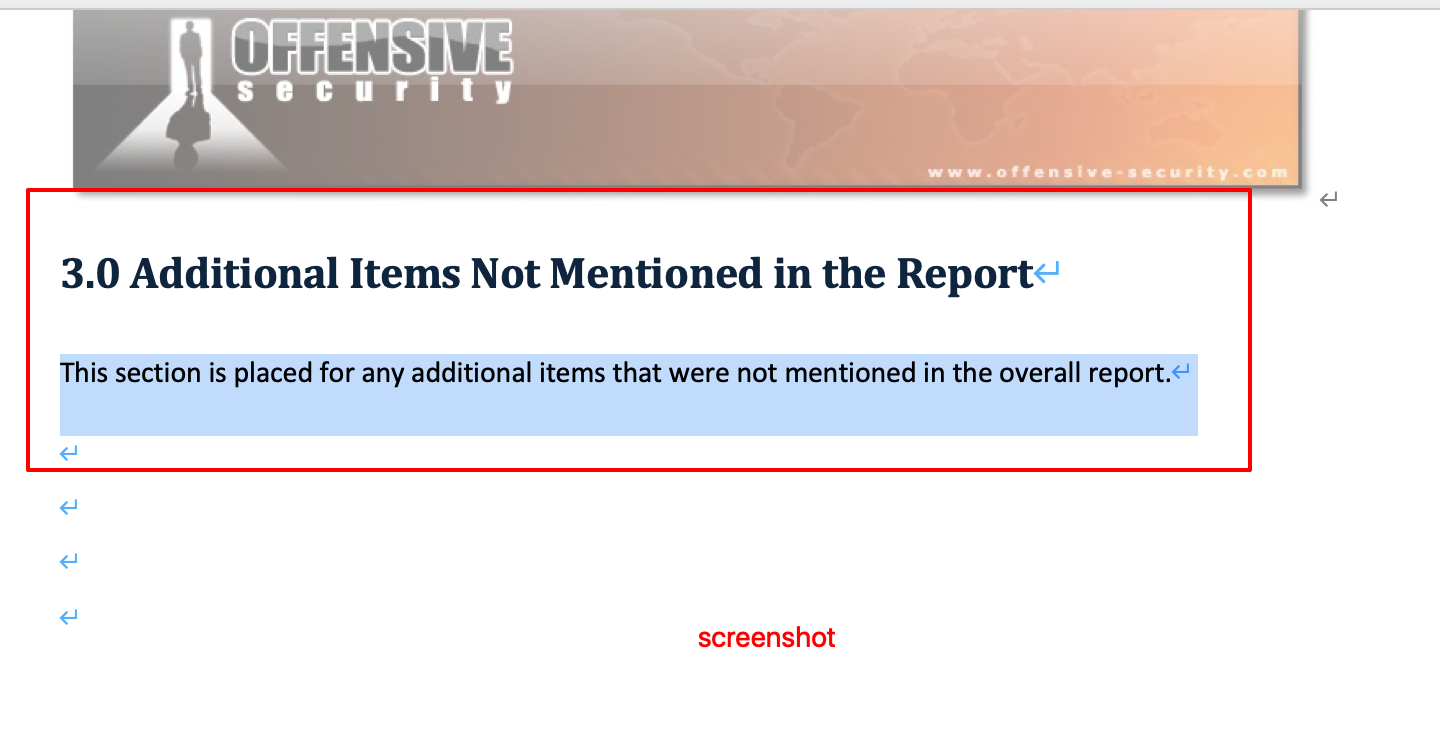
\includegraphics[]{screenshot.png}

\subsection{Steps}
Provide a detailed account of your methodology in creating the exploits. The steps taken should be able to be easily followed and reproducible if necessary.

\section{Additional Items Not Mentioned in the Report}
This section is placed for any additional items that were not mentioned in the overall report.


\end{document}
